\documentclass{beamer}
 
\usepackage[utf8]{inputenc}


\usetheme{Madrid}
\usecolortheme{default}
\usepackage{caption}
\usepackage{subcaption}
\usepackage{hhline}
\usepackage{graphicx}
\usepackage{physics}
\usepackage{amsmath}
\usepackage{amsfonts}
\usepackage{esint}
\usepackage{bbold}
\usepackage{mathtools}
\usepackage{dsfont}
\usepackage{amsthm}
\usepackage{bbm}
\usepackage{amssymb}
\theoremstyle{definition}
\newtheorem{defn}{Definition}[section]
\newtheorem{prop}{Properties}[section]
\newtheorem{rmk}{Remark}[section]
\newtheorem{exmp}{Example}[section]
\newtheorem{prob}{Problem}[section]
\newtheorem{proposition}{Proposition}
\newtheorem{thm}{Theorem}[section]
\newtheorem*{prob*}{Problem}
\newtheorem*{sln*}{Solution}
\usepackage{empheq}
\usepackage{tensor}
\usepackage{MnSymbol,wasysym}

\newcommand{\lag}{\mathcal{L}}
\newcommand{\pOne}{\text{5p}_\text{1/2}}
\newcommand{\pThree}{\text{5p}_\text{3/2}}
\newcommand{\potassium}{^\text{39}\text{K}}
\newcommand{\R}{\mathbb{R}}
\newcommand{\lp}{\left(}
\newcommand{\rp}{\right)}
\newcommand{\lb}{\left[}
\newcommand{\rb}{\right]}
\newcommand{\lc}{\left\{}
\newcommand{\rc}{\right\}}
\newcommand{\p}{\partial}
\newcommand{\f}[2]{\frac{#1}{#2}}
\newcommand{\Vol}{\operatorname{Vol}}
\newcommand{\iprod}{\mathbin{\lrcorner}}
\newcommand{\al}{\alpha}
\newcommand{\be}{\beta}
\newcommand{\FT}{\mathcal{F}}
\newcommand{\LT}{\mathcal{L}}
\usepackage{hyperref}
\usepackage{tensor}
\usepackage{xcolor}
\hypersetup{
	colorlinks,
	linkcolor={black!50!black},
	citecolor={blue!50!black},
	urlcolor={blue!80!black}
}

% 3j symbol
\newcommand{\tj}[6]{ \begin{pmatrix}
		#1 & #2 & #3 \\
		#4 & #5 & #6 
\end{pmatrix}}
% 6j symbol
\newcommand{\Gj}[6]{ \begin{Bmatrix}
		#1 & #2 & #3 \\
		#4 & #5 & #6 
\end{Bmatrix}}

\setbeamerfont{title}{size=\large}

 
 
%Information to be included in the title page:
\title[\textcolor{white}{{}}]
{
	How to make big Hilbert spaces small
}



\author[Bui] % (optional)
{Huan Bui}
\institute[MIT]{} % (optional)
\date{ZGS, Oct 6, 2022}
 
%\logo{
\includegraphics[height=0.3cm]{colby.png}}
 
\begin{document}
 
\frame{\titlepage}

\begin{frame}
	\frametitle{Outline}
	\begin{itemize}
		\item Motivation
		\item Compressing $\ket{\Psi}$ with SVD
		\item Matrix Product States (MPS)
		\item Ground state calculation (roughly)
	\end{itemize}
\end{frame}


\begin{frame}
	\frametitle{Motivation}
	
	$N$ sites, each with spin-$1/2$. Find ground state of:
	\begin{align*}
		\mathcal{H} = - J \sum_{i=1}^N \sigma_i^z \sigma_{i+1}^z - h \sum_{i=1}^N \sigma^x_i
	\end{align*}	
	
	
	Hilbert space dimension: $ 2^N$\\
	
	\vspace{10pt}
	
	Exact diagonalization O.K. for $N \lessapprox 20$ on laptop\\
	
	\vspace{10pt}
	
	$N \to \infty$: needle in the haystack\\
	
	\vspace{10pt}
	
	\pause
	
	{$\boxed{!!}$ For many relevant Hamiltonians, haystack $\ll$ full Hilbert space }\\
	\vspace{5pt}
	{$\quad\,\,\,\,$e.g. haystack $\sim$ subspace of states with low entanglement entropy }\\
	\vspace{5pt}
	{$\quad\,\,\implies$ Clever parameterization + efficient algorithms = \smiley{}?}
	
		
	
\end{frame}



\begin{frame}
	\frametitle{Compressing $\ket{\Psi}$?}
	\begin{align*}
		\ket{\Psi} = \sum_{\{ \sigma \}} \psi_{\sigma_1\sigma_2\dots \sigma_N} \ket{\sigma_1\sigma_2\dots \sigma_N}
	\end{align*}

	\vspace{10pt}
	
	
	\begin{itemize}
		\item \pause How to approximate $\ket{\Psi}$ well without storing $d^N$ coefficients?
		
		\vspace{10pt}
		\item \pause Possible to reduce entanglement entropy after approximation?
	\end{itemize}
\end{frame}


\begin{frame}
	\frametitle{Compressing $\ket{\Psi}$ with SVD}
	
	\begin{theorem}[Singular value decomposition]
		For any $M$, there are unitaries  $U,V$ for which  $M = U S V^\dagger$, with $S = \text{diag}(s_1,s_2,\dots)$.\\
		\vspace{5pt}
		$s_i$: \textit{singular values of} $M \equiv$  eigenvalues of $\sqrt{M^\dagger M }$. $s_i$ $\geq 0$
	\end{theorem}
	
	
	\begin{theorem}[Low-rank approximation]
		The HS-distance from a rank-$m$ matrix $A_{n\times n}$ to the nearest $n\times n$ matrix of rank $k \leq m$  is the square root of the sum of the squares of the smallest $n-k$ singular values of $A$.
	\end{theorem}

	Hilbert-Schmidt norm:
	\begin{align*}
		\norm{A}_{HS} = \sqrt{\sum \abs{A_{ij}}^2} =  \sqrt{\Tr(A^\dagger A)} = \sqrt{\sum s_i^2}
	\end{align*} 
	
\end{frame}



\begin{frame}
	\frametitle{Compressing $\ket{\Psi}$ with SVD}
	
	
	
	\begin{figure}[!htb]
		\centering
		\begin{minipage}{0.45\textwidth}
			\centering
			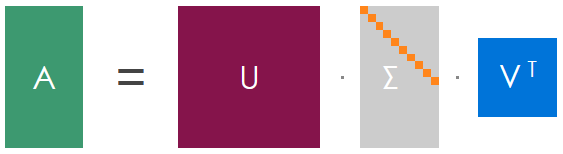
\includegraphics[scale=0.34]{svd1.png}
		\end{minipage}
	$\to$
		\begin{minipage}{0.45\textwidth}
			\centering
			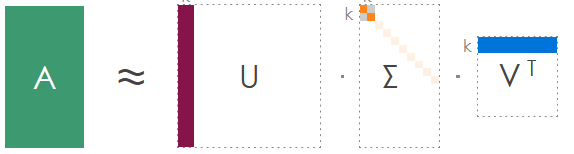
\includegraphics[scale=0.34]{svd2.png}
		\end{minipage}
	\end{figure}

\pause

\vspace{10pt}

\underline{Application}: image compression

\begin{figure}[!htb]
	\centering
	\begin{minipage}{0.45\textwidth}
		\centering
		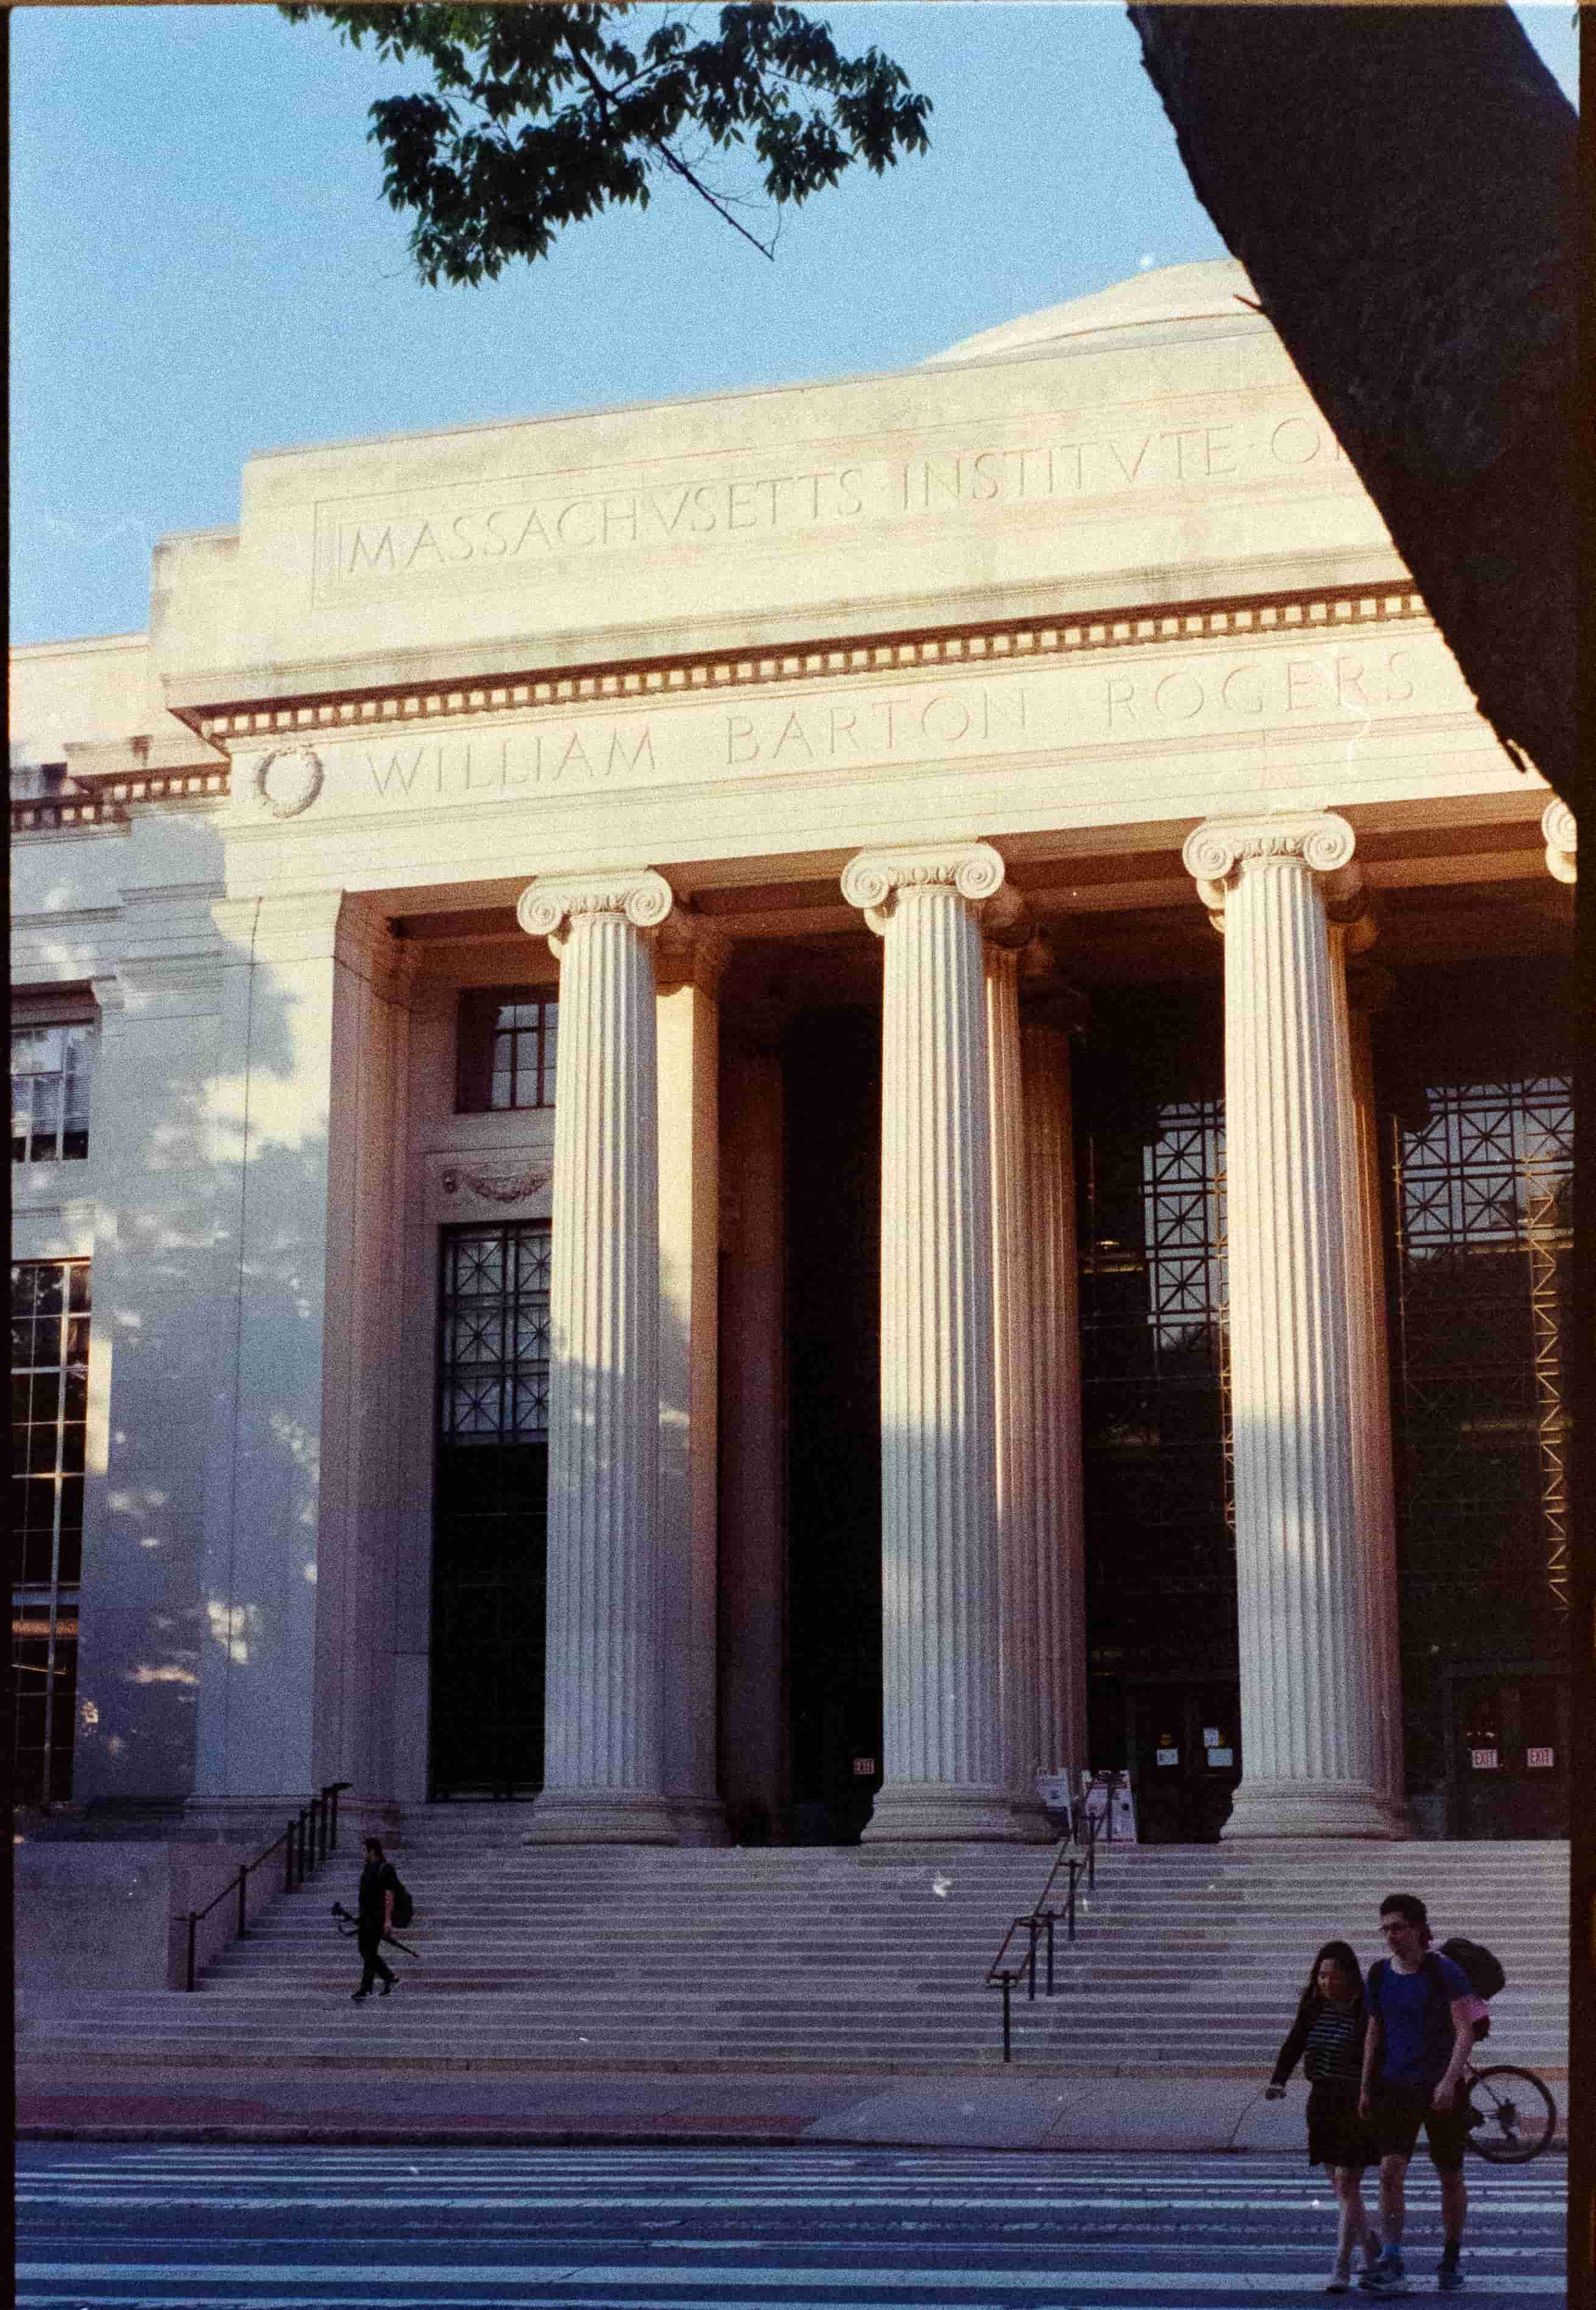
\includegraphics[scale=0.03]{mit.jpg}
	\end{minipage}
	$\to$
	\begin{minipage}{0.45\textwidth}
		\centering
		\includegraphics[scale=0.03]{mit_compressed.png}
	\end{minipage}
\end{figure}
\end{frame}



\begin{frame}
	\frametitle{Compressing $\ket{\Psi}$ with SVD}
	\underline{Idea}: represent $\ket{\Psi}$ as a matrix, then SVD\\
	
	\pause
	
	\vspace{8pt}
	
	Split $N$ spins on a 1d chain into $L+R$: 
	\begin{align*}
		\ket{\Psi} = \sum_{l,r} \psi_{lr} \ket{l}\ket{r}
	\end{align*}
	$\psi_{lr}$ has two indices $\implies$ treat as a matrix (NOT an operator!) \\ 
	
	\pause
	
	\vspace{8pt} 
	
	Apply SVD: $\quad\psi_{lr} = [\mathbf{U}\,\,\mathbf{D}\,\,\mathbf{V}]_{lr}$\\
	
	\vspace{8pt}
	
	$\mathbf{U}, \mathbf{V}$ are unitary. $\mathbf{D} = \text{diag}(s_1,s_2,\dots)$:
	\begin{align*}
		s_i\text{'s} 
		&= \text{singular values of } \psi_{lr} \\
		&= \text{eigenvalues of } \sqrt{\psi^\dagger\psi} = \sqrt{\rho} \implies s_i^2 = \text{eigenvalues of } \rho
	\end{align*}
	
\end{frame}


\begin{frame}
	\frametitle{Compressing $\ket{\Psi}$ with SVD}
	
	After SVD:
	\begin{align*}
		\ket{\Psi} &= \sum_{l,r} \sum_{i} \mathbf{U}_{li}\mathbf{D}_{ii} \mathbf{V}_{ir} \ket{l}\ket{r}\\
		&= \sum_{i} \sum_{\textcolor{blue}{l},\textcolor{red}{r}}  \textcolor{blue}{\mathbf{U}_{li}}\mathbf{D}_{ii} \textcolor{red}{\mathbf{V}_{ir} } \textcolor{blue}{\ket{l}}\textcolor{red}{\ket{r}}\\
		&= \sum_i s_i \ket{i}_L \ket{i}_R \,\,\,\leftarrow \text{ Schmidt decomposition}
	\end{align*}
\pause 
	Can simply read off reduced density matrices:
	\begin{align*}
		\rho_L = \psi\psi^\dagger = \sum_i s_i^2 \ket{i}_L \bra{i}_L \quad\quad\quad \rho_R = \psi^\dagger\psi = \sum_i s_i^2 \ket{i}_R \bra{i}_R
	\end{align*}
\pause
	Normalization:
	\begin{align*}
		\Tr(\psi^\dagger\psi) = \sum_i s_i^2 = 1 \implies s_i^2 \text{: probability for i$^\text{th}$ Schmidt state pair}
	\end{align*}
\end{frame}





\begin{frame}
	\frametitle{Compressing $\ket{\Psi}$ with SVD}
	
	\underline{Example}:  
	\begin{align*}
		\ket{\Psi} = \f{1}{\sqrt{2}}\lp \ket{\uparrow\uparrow} - \ket{\uparrow\downarrow} \rp
	\end{align*}
	\pause 
	Matrixify and SVD:
	\begin{align*}
	\ket{\Psi} = \sum_{ij}\psi_{ij}\ket{i}\ket{j} \quad \text{ with } \quad   [\psi_{ij}] = \begin{pmatrix}
			\f{1}{\sqrt{2}} & -\f{1}{\sqrt{2}} \\ 0 & 0
		\end{pmatrix}
	\end{align*}
\vspace{-10pt}
\pause
\begin{align*}
	[\psi_{ij}] = \begin{pmatrix}
			1 & 0 \\ 0 & 1
		\end{pmatrix}
	\underbrace{\begin{pmatrix}
		1 & 0 \\ 0 & 0 
	\end{pmatrix}}_D
	\begin{pmatrix}
		\f{1}{\sqrt{2}} & -\f{1}{\sqrt{2}} \\ 	\f{1}{\sqrt{2}} & \f{1}{\sqrt{2}}
	\end{pmatrix}
	\end{align*}

\end{frame}


\begin{frame}
	\frametitle{Compressing $\ket{\Psi}$ with SVD}
	
	\underline{Why SVD and Schmidt decomposition?} \\
	
	\vspace{8pt}
	
	$\quad$ SVD compression $\equiv$ make states with low entanglement entropy\\
	
	
	\vspace{8pt} \pause
	
	\underline{How?} von Neumann entanglement entropy between $L$ and $R$:
	\begin{align*}
		S(\rho_L) = -\Tr[\rho_L \ln \rho_L] = -\Tr[\rho_R \ln \rho_R] = S(\rho_R) 
	\end{align*}
\pause
	Eigenvalues of $\rho_L, \rho_R$ are exactly $\{s_i^2\}$.
	\begin{align*}
		\rho_L = \psi\psi^\dagger = \sum_i s_i^2 \ket{i}_L \bra{i}_L \quad\quad\quad \rho_R = \psi^\dagger\psi = \sum_i s_i^2 \ket{i}_R \bra{i}_R
	\end{align*} \pause
So, \vspace{-30pt}
	\begin{align*}
		S = S(\rho_L) = S(\rho_R) = -\sum_i^{\sim 2^{N/2}} s_i^2 \ln s_i^2 \to -\sum_i^m s_i^2 \ln s_i^2
	\end{align*}
\text{\textcolor{blue}{Drop small $s_i$'s $\implies$ reduce $S$ and exponential compression, $m\sim \mathcal{O}(100)$}}
	
\end{frame}


\begin{frame}
	\frametitle{Compressing $\ket{\Psi}$ with SVD}
	
	\underline{Example}:  
	\begin{align*}
		\ket{\Psi} = \f{1}{\sqrt{2}}\lp \ket{\uparrow\uparrow} - \ket{\uparrow\downarrow} \rp
	\end{align*}
	Matrixify and SVD
	\begin{align*}
		&\ket{\Psi} = \sum_{ij}\psi_{ij}\ket{i}\ket{j} \quad \text{ with } \quad   [\psi_{ij}] = \begin{pmatrix}
			\f{1}{\sqrt{2}} & -\f{1}{\sqrt{2}} \\ 0 & 0
		\end{pmatrix}\\
		&\quad\quad \,\,\,[\psi_{ij}] = \begin{pmatrix}
			1 & 0 \\ 0 & 1
		\end{pmatrix}
		\underbrace{\begin{pmatrix}
				1 & 0 \\ 0 & 0 
		\end{pmatrix}}_D
		\begin{pmatrix}
			\f{1}{\sqrt{2}} & -\f{1}{\sqrt{2}} \\ 	\f{1}{\sqrt{2}} & \f{1}{\sqrt{2}}
		\end{pmatrix}
	\end{align*}
	\pause Entanglement entropy is 0 $\implies$ not entangled (makes sense)
\end{frame}



\begin{frame}
	\frametitle{But wait...}
		
	We need $\ket{\Psi}$ to compress. But we want to find such a $\ket{\Psi}$ for some $H$. \\
	
	\pause
	
	\vspace{15pt}
	
	\begin{figure}[!htb]
		\centering
		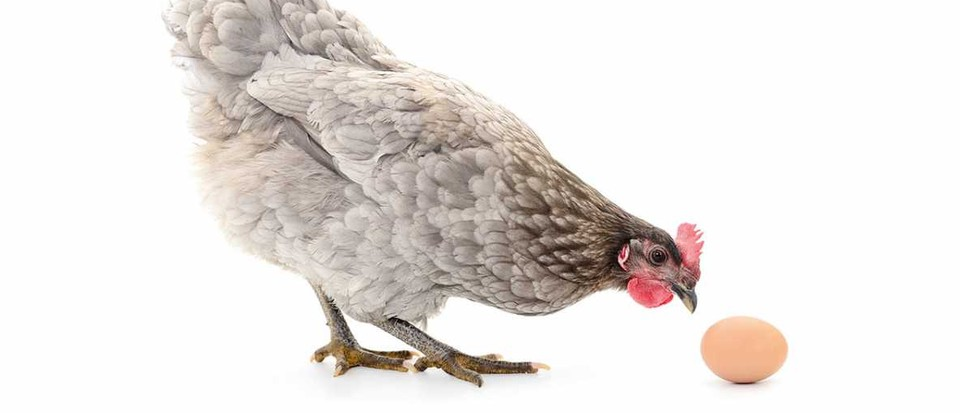
\includegraphics[scale=0.2]{chickenegg.jpg}
	\end{figure}
	
	\vspace{8pt}

\end{frame}





\begin{frame}
	\frametitle{MPS and DMRG}
	MPS: Matrix product state $\,\,\leftarrow$ \\
	
	\vspace{8pt}
	
	DMRG: Density matrix renormalization group\\
	
	\vspace{8pt}
	
	\pause
	
	
	\vspace{12pt}
	
	MPS: 
	\begin{itemize}
		\item expresses wavefunctions as products of matrices
		
		\item natural way to generate states with low entanglement entropy
	\end{itemize}
\pause

	DMRG:
	\begin{itemize}
		\item numerical variational technique for finding ground states
		
		\item works with MPS, not $\ket{\Psi}$
		
		\item most efficient method for 1d systems
	\end{itemize}
	
	
\end{frame}



\begin{frame}
	\frametitle{MPS}
	\textbf{Every $\ket{\Psi}$ can be written as an MPS.} From Schmidt decomposition:
	\begin{align*}
		\ket{\Psi} = \sum_{i} s_i \ket{i}_L \ket{i}_R = \sum_{i_m} s_i \ket{i_m}_L \ket{i_m}_R
	\end{align*}
	$m:$ position on the 1d chain where the $L-R$ split occurs. \\
	
	\vspace{15pt}
	\pause
	
	\underline{$\ket{i_m}_L$ can be built recursively}:
	\begin{align*}
		&\ket{i_1}_L = \sum_{\sigma_1}A^{\sigma_1}_{i_1}\ket{\sigma_1}\\ 
		&\textcolor{white}{\ket{i_2}_L = \sum_{i_1,\sigma_2} A^{\sigma_2}_{i_2,i_1}  \ket{i_1}_L \ket{\sigma_2} = \sum_{i_1,\sigma_1,\sigma_2} A^{\sigma_1}_{i_1}   A^{\sigma_2}_{i_2,i_1} \ket{\sigma_1\sigma_2} = \sum_{\sigma_1,\sigma_2} (A^{\sigma_1}A^{\sigma_2})_{1,i_2} \ket{\sigma_1\sigma_2}}\\
		&\textcolor{white}{\ket{i_3}_L = \sum_{\sigma_1,\sigma_2,\sigma_3}(A^{\sigma_1}A^{\sigma_2}A^{\sigma_3})_{1,i_3} \ket{\sigma_1\sigma_2\sigma_3}}\\
		&\textcolor{white}{\quad\vdots}
	\end{align*}
\end{frame}


\begin{frame}
	\frametitle{MPS}
	\textbf{Every $\ket{\Psi}$ can be written as an MPS.} From Schmidt decomposition:
	\begin{align*}
		\ket{\Psi} = \sum_{i} s_i \ket{i}_L \ket{i}_R = \sum_{i_m} s_i \ket{i_m}_L \ket{i_m}_R
	\end{align*}
	$m:$ position on the 1d chain where the $L-R$ split occurs. \\
	
	\vspace{15pt}
	
	\underline{$\ket{i_m}_L$ can be built recursively}:
	\begin{align*}
		&\ket{i_1}_L = \sum_{\sigma_1}A^{\sigma_1}_{i_1}\ket{\sigma_1}\\ 
		&\textcolor{black}{\ket{i_2}_L = \sum_{i_1,\sigma_2} A^{\sigma_2}_{i_2,i_1}  \ket{i_1}_L \ket{\sigma_2} = \sum_{i_1,\sigma_1,\sigma_2} A^{\sigma_1}_{i_1}   A^{\sigma_2}_{i_2,i_1} \ket{\sigma_1\sigma_2} = \sum_{\sigma_1,\sigma_2} (A^{\sigma_1}A^{\sigma_2})_{1,i_2} \ket{\sigma_1\sigma_2}}\\
		&\textcolor{white}{\ket{i_3}_L = \sum_{\sigma_1,\sigma_2,\sigma_3}(A^{\sigma_1}A^{\sigma_2}A^{\sigma_3})_{1,i_3} \ket{\sigma_1\sigma_2\sigma_3}}\\
		&\textcolor{white}{\quad\vdots}
	\end{align*}
\end{frame}


\begin{frame}
	\frametitle{MPS}
	\textbf{Every $\ket{\Psi}$ can be written as an MPS.} From Schmidt decomposition:
	\begin{align*}
		\ket{\Psi} = \sum_{i} s_i \ket{i}_L \ket{i}_R = \sum_{i_m} s_i \ket{i_m}_L \ket{i_m}_R
	\end{align*}
	$m:$ position on the 1d chain where the $L-R$ split occurs. \\
	
	\vspace{15pt}
	
	\underline{$\ket{i_m}_L$ can be built recursively}:
	\begin{align*}
		&\ket{i_1}_L = \sum_{\sigma_1}A^{\sigma_1}_{i_1}\ket{\sigma_1}\\ 
		&\textcolor{black}{\ket{i_2}_L = \sum_{i_1,\sigma_2} A^{\sigma_2}_{i_2,i_1}  \ket{i_1}_L \ket{\sigma_2} = \sum_{i_1,\sigma_1,\sigma_2} A^{\sigma_1}_{i_1}   A^{\sigma_2}_{i_2,i_1} \ket{\sigma_1\sigma_2} = \sum_{\sigma_1,\sigma_2} (A^{\sigma_1}A^{\sigma_2})_{1,i_2} \ket{\sigma_1\sigma_2}}\\
		&\textcolor{black}{\ket{i_3}_L = \sum_{\sigma_1,\sigma_2,\sigma_3}(A^{\sigma_1}A^{\sigma_2}A^{\sigma_3})_{1,i_3} \ket{\sigma_1\sigma_2\sigma_3}}\\
		&\textcolor{black}{\quad\vdots}
	\end{align*}
\end{frame}





\begin{frame}
	\frametitle{MPS}
	Schmidt states:
	\begin{align*}
		&\ket{i_m}_L = \sum_{\{\sigma\}_1^m} (A^{\sigma_1}A^{\sigma_2}\dots A^{\sigma_m})_{1,i_m}  \ket{\sigma_1 \sigma_2\dots\sigma_m} \\
		&\ket{i_m}_R = \sum_{\{\sigma\}_{m+1}^N} (B^{\sigma_{m+1}}B^{\sigma_{m+2}}\dots B^{\sigma_N})_{i_m,1}  \ket{\sigma_{m+1}\sigma_{m+2}\dots\sigma_N} 
	\end{align*}
	\pause
	Full wavefunction:
	\begin{align*}
		\boxed{\ket{\Psi} = \sum_{\{\sigma\}}    A^{\sigma_1}A^{\sigma_2}\dots A^{\sigma_m}  \,\,{S}\,\, B^{\sigma_{m+1}}B^{\sigma_{m+2}}\dots B^{\sigma_N}  \ket{\sigma_1\sigma_2\dots \sigma_N}}
	\end{align*}
	Matrix dimensions:
	\begin{align*}
		\underbrace{(1\times d), (d\times d^2), \dots }_{A}, \underbrace{(d^{N/2}\times d^{N/2})}_{S},  \underbrace{\dots (d^2\times d), (d\times 1)}_{B}
	\end{align*}


\end{frame}



\begin{frame}
	\frametitle{MPS}
	
	\underline{Example}: 
	\begin{align*}
		\ket{\text{GHZ}_4} = \f{\ket{0000} + \ket{1111}}{\sqrt{2}}= \f{1}{\sqrt{2}}
		\sum_{\{\sigma\}} A_1^{\sigma_1} A_2^{\sigma_2} A_3^{\sigma_3} A_4^{\sigma_4}  \ket{\sigma_1\sigma_2\sigma_3\sigma_4}
	\end{align*}\pause
	where 
	\begin{align*}
		A^{0}_1 =\begin{pmatrix}
			1 & 0
		\end{pmatrix}, \,\,\,\,
	A^{0}_2 = \begin{pmatrix}
		1 & 0 & 0 & 0 \\ 0 & 0 & 0 & 0
	\end{pmatrix}, \,\,\,\,
	A^{0}_3 = \begin{pmatrix}
		1 & 0 \\ 0 & 0 \\ 0 & 0 \\ 0 & 0
	\end{pmatrix},\,\,\,\,
	A^{0}_4 = \begin{pmatrix}
		1 \\ 0 
	\end{pmatrix}
	\end{align*}
\vspace{-20pt}
\begin{align*}
	A^{1}_1 =\begin{pmatrix}
		0 & 1
	\end{pmatrix}, \,\,\,\,
	A^{1}_2 = \begin{pmatrix}
		0 & 0 & 0 & 0 \\ 0 & 0 & 0 & 1
	\end{pmatrix}, \,\,\,\,
	A^{1}_3 = \begin{pmatrix}
		0 & 0 \\ 0 & 0 \\ 0 & 0 \\ 0 & 1
	\end{pmatrix},\,\,\,\,
	A^{1}_4 = \begin{pmatrix}
		0 \\ 1
	\end{pmatrix}
\end{align*}
\end{frame}




\begin{frame}
	\frametitle{MPS \& Hilbert space decimation}
	\underline{Idea}: Motivated by SVD, not allow matrix dimensions to exceed a fixed $D$\\ \pause
	
	\vspace{10pt}
	
	From:
	\begin{align*}
		{(1\times d), (d\times d^2), \dots }, {(d^{N/2}\times d^{N/2})},  {\dots (d^2\times d), (d\times 1)}
	\end{align*}
	To:
	\begin{align*}
		{(1\times d), (d\times d^2), \dots (D\times D)}, {(D \times D)},  { (D\times D)\dots (d^2\times d), (d\times 1)}
	\end{align*}
	
	\vspace{10pt} \pause
	
	To generalize, can make all matrices to $D\times D$, so that
	\begin{align*}
		\boxed{\ket{\Psi} = \sum_{\{\sigma\}}   \Tr\lb  A_{\textcolor{gray}{1}}^{\sigma_1}A_{\textcolor{gray}{2}}^{\sigma_2}\dots A_{\textcolor{gray}{m}}^{\sigma_m}  A_{{\textcolor{gray}{m+1}}}^{\sigma_{m+1}}A_{{\textcolor{gray}{m+2}}}^{\sigma_{m+2}}\dots A_{\textcolor{gray}{N}}^{\sigma_N} \rb  \ket{\sigma_1\sigma_2\dots \sigma_N}}
	\end{align*}
	
	
	
\end{frame}


\begin{frame}
	\frametitle{MPS}
		\underline{Example}: 
	\begin{align*}
		\ket{\text{GHZ}_4} = \f{\ket{0000} + \ket{1111}}{\sqrt{2}}= \f{1}{\sqrt{2}}
		\sum_{\{\sigma\}} \Tr \lb  A^{\sigma_1} A^{\sigma_2} A^{\sigma_3} A^{\sigma_4} \rb \ket{\sigma_1\sigma_2\sigma_3\sigma_4}
	\end{align*} 
\pause
	where
	\begin{align*}
		A^0 = \begin{pmatrix}
			1 & 0 \\ 0 & 0 
		\end{pmatrix} \quad\quad \quad 
	A^1 = \begin{pmatrix}
		0 & 0 \\ 0 & 1
	\end{pmatrix}
	\end{align*}
	Can see that
	\begin{align*}
		\Tr \lb  A^{\sigma_1} A^{\sigma_2} A^{\sigma_3} A^{\sigma_4} \rb = 1 \iff \sigma_1 = \sigma_2 = \sigma_3 = \sigma_4
	\end{align*}
	
\end{frame}


\begin{frame}
	\frametitle{So far}
	\begin{itemize}
		\item SVD \& Schmidt decomposition allows for compressing $\ket{\Psi}$ 
		\vspace{10pt} \pause
		
		\item From Schmidt decomposition to MPS for general $\ket{\Psi}$
		\vspace{10pt} \pause
		
		\item Decimate Hilbert space by keeping matrices in MPS at $(D\times D)$
		\vspace{10pt} \pause
		
		\item Smaller Hilbert space ($ND^2 \text{ vs } d^N$) and MPS  corresponds to $\ket{\Psi}$ with lower entanglement entropy
		\vspace{10pt} \pause
		
		\item MPS: natural way to describe ground states of relevant Hamiltonians 
	\end{itemize}
	
\end{frame}


\begin{frame}
	\frametitle{Graphical notation}
	Matrices:
	\vspace{-10pt}
	\begin{figure}[!htb]
		\centering
		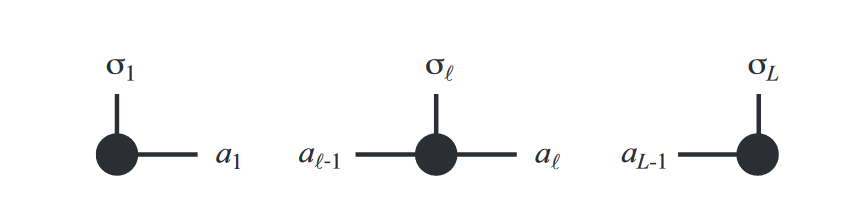
\includegraphics[scale=0.3]{matrix.png}
	\end{figure}
\vspace{-10pt}
	MPS:
	\vspace{-10pt}
	\begin{figure}[!htb]
		\centering
		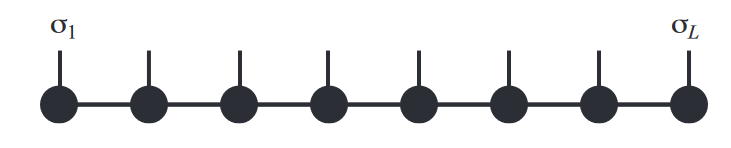
\includegraphics[scale=0.32]{mps.png}
	\end{figure}
	Overlap for two MPS's (arrows indicate sum over indices)
	\vspace{-6pt}
	\begin{figure}[!htb]
		\centering
		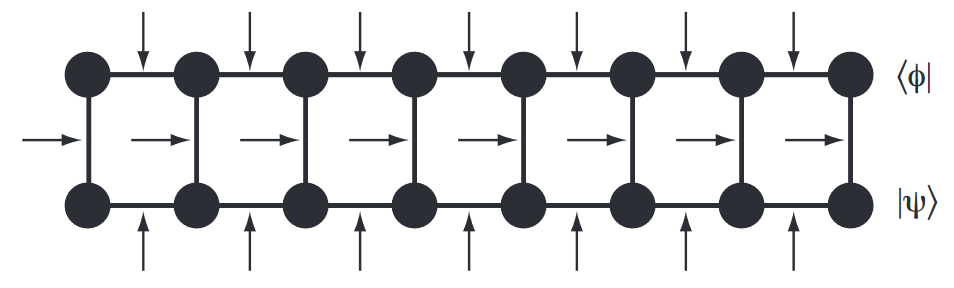
\includegraphics[scale=0.28]{overlap.png}
	\end{figure}
\end{frame}



\begin{frame}
	\frametitle{Graphical notation}
	\underline{MPO}: Matrix product operators \\
	
	\vspace{10pt}
	If $\bra{\sigma_1\sigma_2\dots \sigma_N} \ket{\Psi} = A^{\sigma_1}A^{\sigma_2}\dots A^{\sigma_N}$, then
	\begin{align*}
		\bra{\sigma_1\dots \sigma_N} \hat{O} |\sigma_1'\dots \sigma_N'\rangle = W^{\sigma_1\sigma'_1}W^{\sigma_2\sigma'_2}\dots W^{\sigma_{N-1}\sigma'_{N-1}}W^{\sigma_N\sigma'_N}
	\end{align*} 
	or \pause
	\begin{align*}
		\hat{O} = \sum_{\{\sigma,\sigma'\}} W^{\sigma_1\sigma'_1}W^{\sigma_2\sigma'_2}\dots W^{\sigma_{N-1}\sigma'_{N-1}}W^{\sigma_N\sigma'_N} \ket{\sigma}\langle \sigma'|
	\end{align*}
	$\implies$ can calculate $\bra{\Psi} H \ket{\Psi}$ in MPS language
\end{frame}

\begin{frame}
	\frametitle{Graphical notation}
	MPO on MPS:
	\begin{align*}
		\hat{O}\ket{\Psi} 
		= \sum_{\{\sigma,\sigma'\}} (W^{\sigma_1\sigma_1'}W^{\sigma_2\sigma_2'}\dots)(A^{\sigma_1}A^{\sigma_2}\dots) \ket{\sigma} 
		= \sum_{\{\sigma\}} N^{\sigma_1}N^{\sigma_2}\dots \ket{\sigma}
 	\end{align*}
 	\begin{figure}[!htb]
 		\centering
 		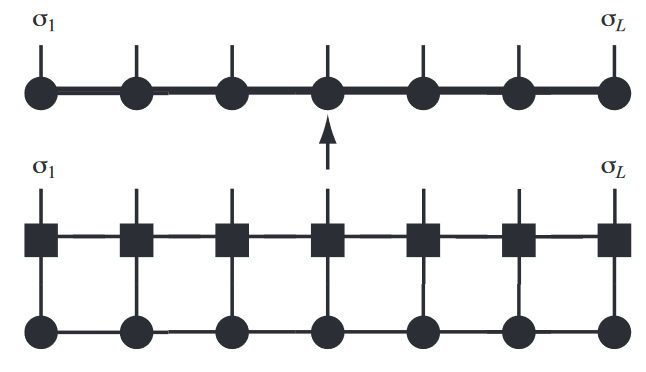
\includegraphics[scale=0.3]{mpo_on_mps.png}
 	\end{figure}
\end{frame}




\begin{frame}
	\frametitle{Ground state search}
	Variationally extremize 
	\begin{align*}
		\bra{\Psi} H \ket{\Psi} - \lambda \braket{\Psi}, \text{ so that }  \ket{\Psi} \to \ket{\Psi_g},\,\, \lambda \to E_0
	\end{align*}

	
	\vspace{10pt}
	
	\pause
	
	Graphically,
	\begin{figure}[!htb]
		\centering
		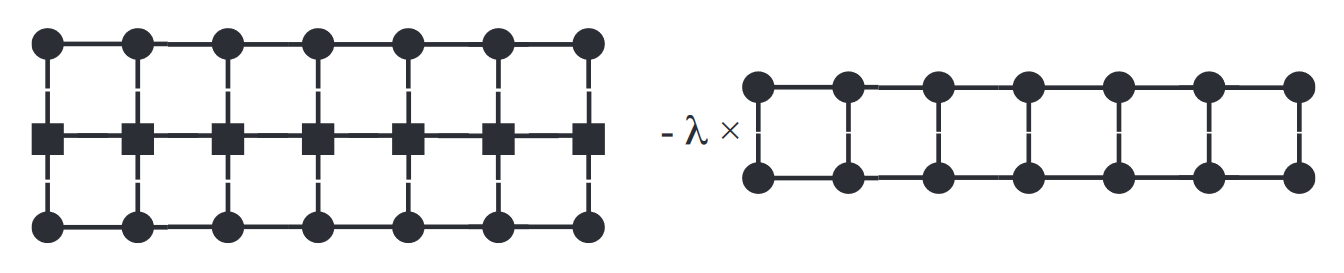
\includegraphics[scale=0.3]{gnd_state_search.png}
	\end{figure}
	\underline{Idea}: Keep matrices on all sites but one $(\ell)$ constant, optimize elements of $M^{\sigma_\ell}_{\ell}$. Sweep through $\ell$.
\end{frame}


\begin{frame}
	\frametitle{Ground state search}
	Minimizing
	\begin{figure}[!htb]
		\centering
		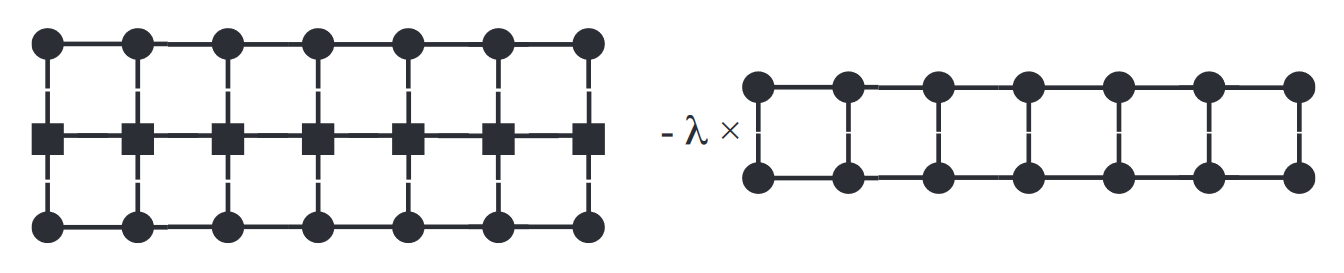
\includegraphics[scale=0.25]{gnd_state_search.png}
	\end{figure}
	$\equiv$ solving (gradient descent)
	\begin{figure}[!htb]
		\centering
		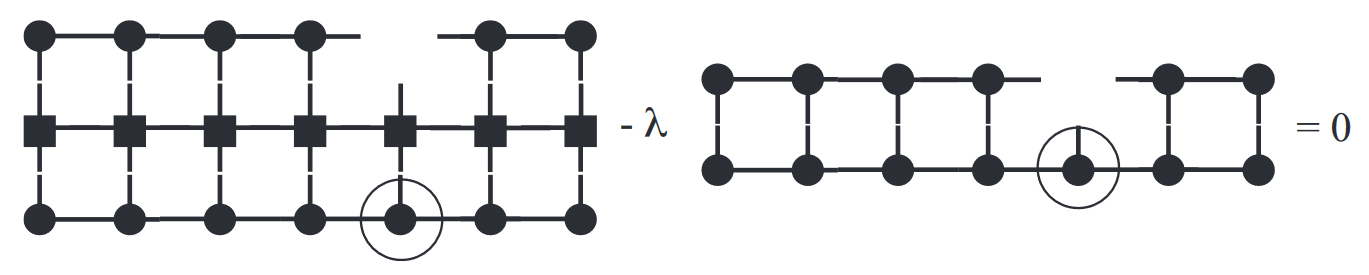
\includegraphics[scale=0.25]{gnd_state_search1.png}
	\end{figure}
	$\implies$ a generalized eigenvalue problem, where we treat $M^{\sigma_\ell}_\ell$ as a vector $v$
\end{frame}

\begin{frame}
	\frametitle{Ground state search}
	
	\underline{Aside}: left-/right-normalized
	\begin{align*}
		\sum_{\sigma_\ell} A^{\sigma_\ell\dagger} A^{\sigma_\ell} = I \quad\quad \sum_{\sigma_\ell} B^{\sigma_\ell\dagger} B^{\sigma_\ell} = I
	\end{align*}
	
	If $\ket{\Psi}$ is both left- and right-normalized,
	\begin{figure}[!htb]
		\centering
		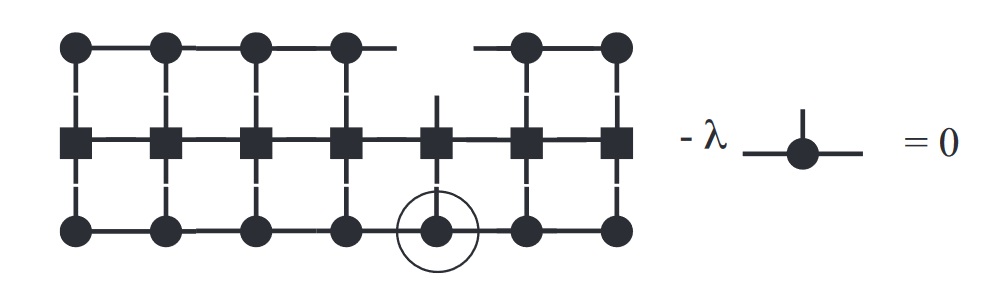
\includegraphics[scale=0.25]{gnd_state_search2.png}
\end{figure}
	$\implies$ standard eigenvalue problem 
\end{frame}


\begin{frame}
	\frametitle{Ground state search}
	Algorithm: \vspace{5pt}
	\begin{itemize}
		\item Start with initial guess for $\ket{\Psi}$, which is right-normalized $\ket{\Psi} \sim BBBBB\dots$ \pause
		\vspace{5pt}
		\item Calculate current state of network for sites $N-1$ through $1$ \pause
		\vspace{5pt}
		\item \textit{Right-sweep}: From $\ell=1$ through $N-1$: at $\ell$, solve for $M^{\sigma_\ell}$ then left-normalize into $A^{\sigma_\ell}$ by SVD; remaining matrices of the SVD are multiplied into $M^{\sigma_{\ell+1}}$  \pause
		\vspace{5pt}
		
		\item \textit{Left-sweep}: From $\ell=L$ through $\ell=2$: at $l$, solve for $M^{\sigma_\ell}$ then right-normalize into $B^{\sigma_\ell}$ by SVD; remaining matrices of the SVD are multiplied into $M^{\sigma_{\ell-1}}$
		\vspace{5pt} \pause
		
		\item Repeat right and left sweeps until convergence
	\end{itemize}
\end{frame}


\begin{frame}
	\frametitle{Ground state search}
	
	Algorithm, formalized: Subscript denotes the number of updates
	\begin{align*}
		M_0 B_0 B_0 B_0 &\xrightarrow{\text{diag}} M_1 B_0 B_0 B_0  \xrightarrow{\text{SVD}} A_1 M_0 B_0 B_0  \\
		&\xrightarrow{\text{diag}} A_1 M_1 B_0 B_0  \xrightarrow{\text{SVD}} A_1 A_1 M_0 B_0  \\
		&\xrightarrow{\text{diag}} A_1 A_1 M_1 B_0  \xrightarrow{\text{SVD}} A_1 A_1 A_1 M_0  \\
		&\xrightarrow{\text{diag}} A_1 A_1 A_1 M_1  \xrightarrow{\text{SVD}} A_1 A_1 M_1 B_1  \\
		&\xrightarrow{\text{diag}} A_1 A_1 M_2 B_1  \xrightarrow{\text{SVD}} A_1 M_1 B_2 B_1  \\
		&\xrightarrow{\text{diag}} A_1 M_2 B_2 B_1   \xrightarrow{\text{SVD}} M_1 B_2 B_2 B_1  \\
		&\quad\vdots
	\end{align*}
	
\end{frame}

\begin{frame}

\frametitle{DMRG}

\pause
\begin{itemize}
\item Introduce left and right blocks $A$ and $B$, with one spin in each \pause
\vspace{8pt}
\item Insert a pair between $A$ and $B$, so chain looks like $A \circ \circ B$ \pause
\vspace{8pt}
\item Diagonalize Hamiltonian to get $\ket{\Psi_0}$ and $E_0$ \pause
\vspace{8pt}
\item Find reduced Hilbert space for $A\circ$ and $\circ B$. How? \vspace{5pt}  \pause
	\begin{itemize}
	\item Schmidt-decompose $\ket{\Psi_0}$ and truncate \vspace{5pt}
	\item Get approximate $\ket{\tilde{\psi}_0}$ with rank $D$ (out of $Dd$) \vspace{5pt}\\
	$\implies$  $D$ most relevant states in $A\circ$, same for $\circ B$
	\end{itemize} 
	\vspace{8pt} \pause
\item Repeat
\end{itemize}
\end{frame}


\begin{frame}
\frametitle{DMRG}
\begin{figure}[!htb]
\centering
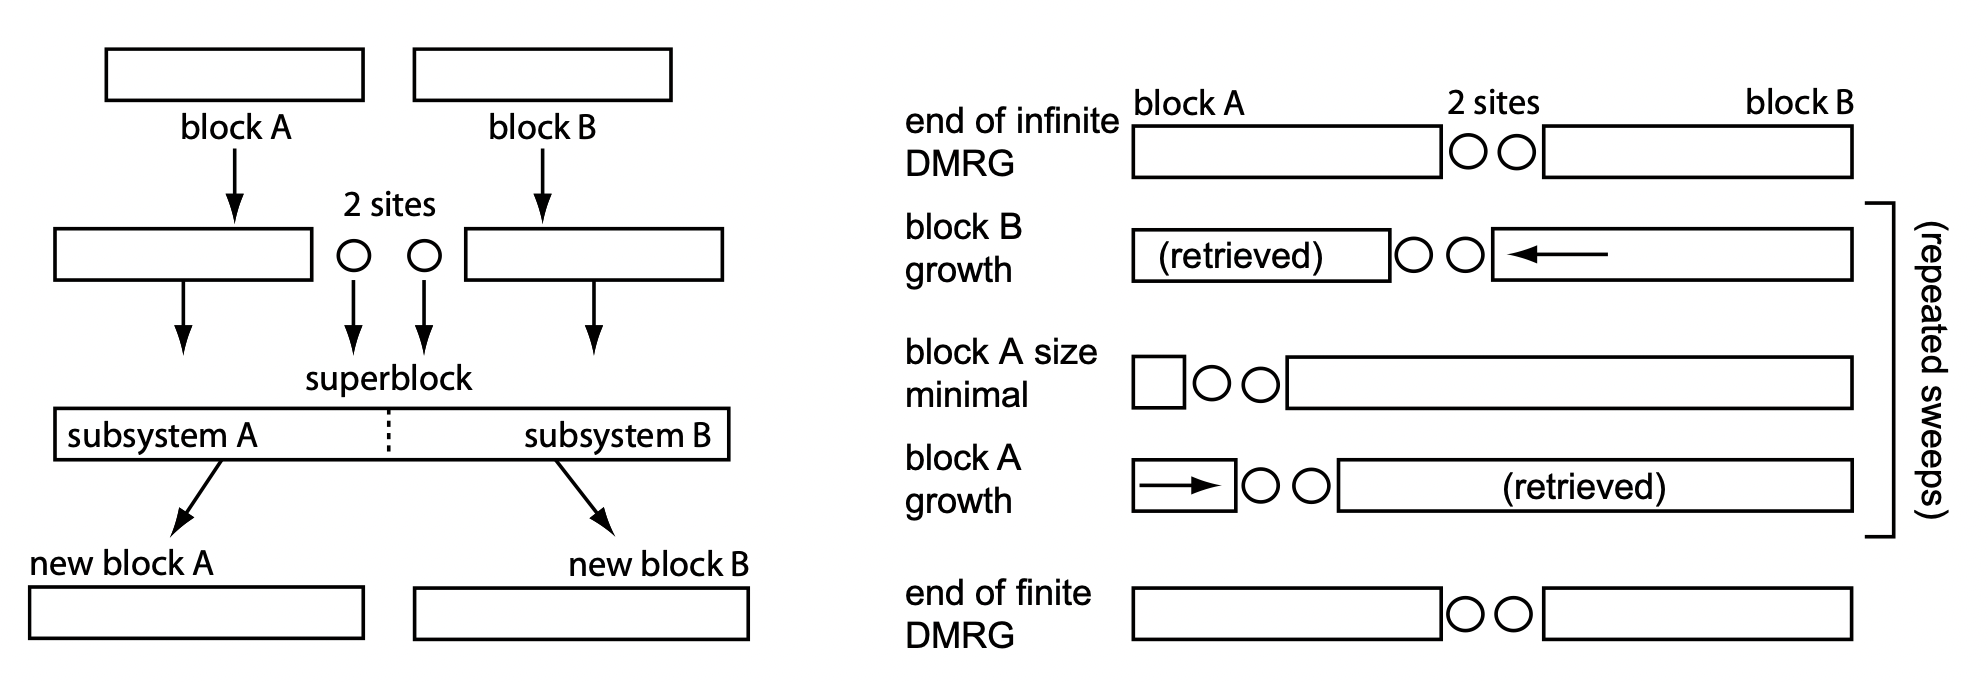
\includegraphics[scale=0.33]{DMRG.PNG}
\end{figure}
\end{frame}

\begin{frame}
	\frametitle{References}
	
	\nocite{*}
	\bibliographystyle{unsrt}
	\bibliography{references}
\end{frame}



\end{document}